\chapter{System Design}
\section{System Architecture}
\begin{figure}[H] % 'H' means force placement here
    \centering
    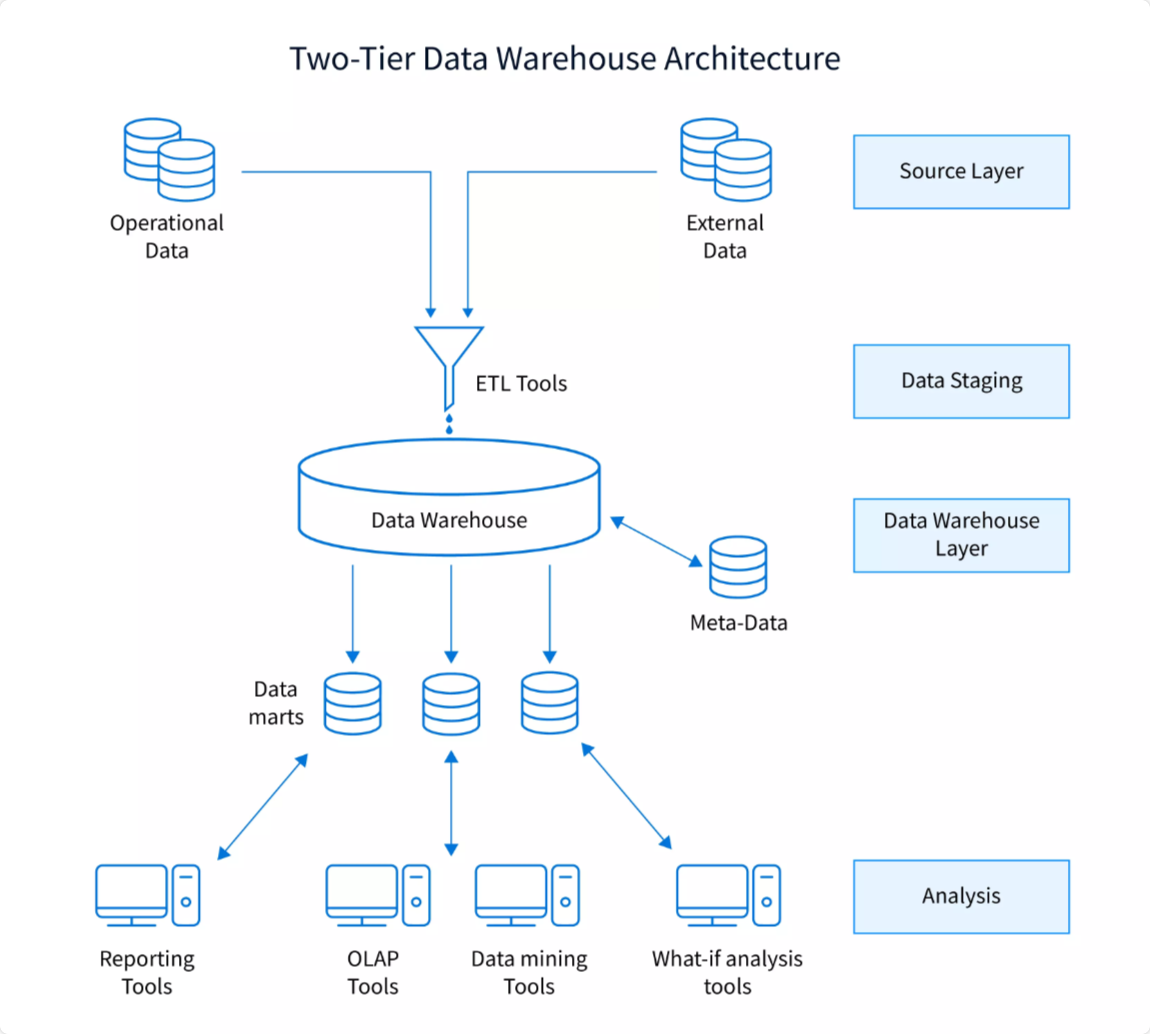
\includegraphics[width=0.7\textwidth]{images/unnamed.png} 
    \caption{System Architecture Diagram.}
    \label{fig:my_label} % For referencing in text
\end{figure}
\section{Data Flow Diagram}
\begin{figure}[H] % 'H' means force placement here
    \centering
    \includegraphics[width=0.7\textwidth]{images/imagename.jpg} 
    \caption{Data Flow Diagram}
    \label{fig:my_label} % For referencing in text
\end{figure}
\section{UML Diagrams}
\subsection{Class Diagram}
\begin{figure}[H] % 'H' means force placement here
    \centering
    \includegraphics[width=0.7\textwidth]{images/imagename.jpg} 
    \caption{Class Diagram}
    \label{fig:my_label} % For referencing in text
\end{figure}
\subsection{Object Diagram}
\begin{figure}[H] % 'H' means force placement here
    \centering
    \includegraphics[width=0.7\textwidth]{images/imagename.imageformat(like jpg or png)} 
    \caption{Object Diagram}
    \label{fig:my_label} % For referencing in text
\end{figure}
\subsection{Collaboration Diagram}
\begin{figure}[H] % 'H' means force placement here
    \centering
    \includegraphics[width=0.7\textwidth]{images/imagename.imageformat(like jpg or png)} 
    \caption{Collaboration Diagram}
    \label{fig:my_label} % For referencing in text
\end{figure}
\subsection{Use Case Diagram}
\begin{figure}[H] % 'H' means force placement here
    \centering
    \includegraphics[width=0.7\textwidth]{images/imagename.imageformat(like jpg or png)} 
    \caption{Use Case Diagram}
    \label{fig:my_label} % For referencing in text
\end{figure}
\subsection{Sequence Diagram}
\begin{figure}[H] % 'H' means force placement here
    \centering
    \includegraphics[width=0.7\textwidth]{images/imagename.imageformat(like jpg or png)} 
    \caption{Sequence Diagram}
    \label{fig:my_label} % For referencing in text
\end{figure}
\subsection{Activity Diagram}
\begin{figure}[H] % 'H' means force placement here
    \centering
    \includegraphics[width=0.7\textwidth]{images/imagename.imageformat(like jpg or png)} 
    \caption{Activity Diagram}
    \label{fig:my_label} % For referencing in text
\end{figure}
\subsection{Component Diagram}
\begin{figure}[H] % 'H' means force placement here
    \centering
    \includegraphics[width=0.7\textwidth]{images/imagename.imageformat(like jpg or png)} 
    \caption{Component Diagram}
    \label{fig:my_label} % For referencing in text
\end{figure}
\subsection{Deployment Diagram}
\begin{figure}[H] % 'H' means force placement here
    \centering
    \includegraphics[width=0.7\textwidth]{images/imagename.imageformat(like jpg or png)} 
    \caption{Deployment Diagram}
    \label{fig:my_label} % For referencing in text
\end{figure}
